% -*- root: ../gvoysey-thesis.tex -*-
\chapter{Methods}
\label{chapter:Methods}
\thispagestyle{myheadings}

% set this to the location of the figures for this chapter. it may
% also want to be ../Figures/2_Body/ or something. make sure that
% it has a trailing directory separator (i.e., '/')!
\graphicspath{{4_Methods/Figures/}}

\section{Chapter Summary} % (fold)
\label{sec:methodsummary}
This chapter gives a detailed description of the modeling environment created for this thesis.  \hyperref[sec:overview_of_modeling_framework]{First}, the configuration of the overall system is detailed.  \hyperref[sec:peripheral_models]{Second}, the configuration and use of two models of the auditory periphery are detailed.  \hyperref[sec:auditory_nerve_response_models]{Third}, the creation of compound action potentials and population responses of the auditory nerve are given.  A method for the simulation of cochlear synaptopathy is also detailed, along with a new incorporation of a nonlinear distribution of auditory nerve fiber types as a function of center frequency.  \hyperref[sec:brainstem_models]{Fourth}, the use of these auditory nerve responses in simulation of the auditory brainstem and midbrain with two models are given, culminating in the creation of modeled Auditory Brainstem Responses.  \hyperref[sub:automated_parameter_exploration]{Finally}, the utility of the system for large-scale simulation is shown. 
% section methodsummary (end)

\section{Overview of Modeling Framework} % (fold)
\label{sec:overview_of_modeling_framework}
The modeling framework created for this thesis has been named Corti\citep{Voysey2016Corti}. It is architecturally inspired by the EarLab project developed at Boston University as well as the Cochlea\citep{Rudnicki2014Cochlea} modeling environment developed at the Technical University of Munich, from which it incorporates a peripheral model.

Corti is a command-line tool written in Python. As detailed in \autoref{fig:corti-overview}, it is designed to produce estimates of the Auditory Brainstem Response, auditory nerve fiber, auditory nerve, brainstem and midbrain responses to an arbitrary stimulus.  A set of configuration parameters define which models are used and how they are interconnected, as well as the spatiotemporal properties of the stimulus.

\subsection{Configuration options define a parameter space}
As detailed in \autoref{chapter:literaturereview}, the constituent models of this framework each require many choices of parameters, ranging from sampling frequency to the time constants and relative inhibitory and excitatory contributions of brainstem areas. Several other parameters are introduced in the framework itself, as well as the choice of which model to use for each stage. Because these parameter choices directly modulate the simulation output, it quickly becomes natural to treat these different options as a high-dimensional parameter space.  Any single run of the framework, using one collection of options, defines a particular trajectory though this space.

\begin{figure}[htbp]
	\centering
	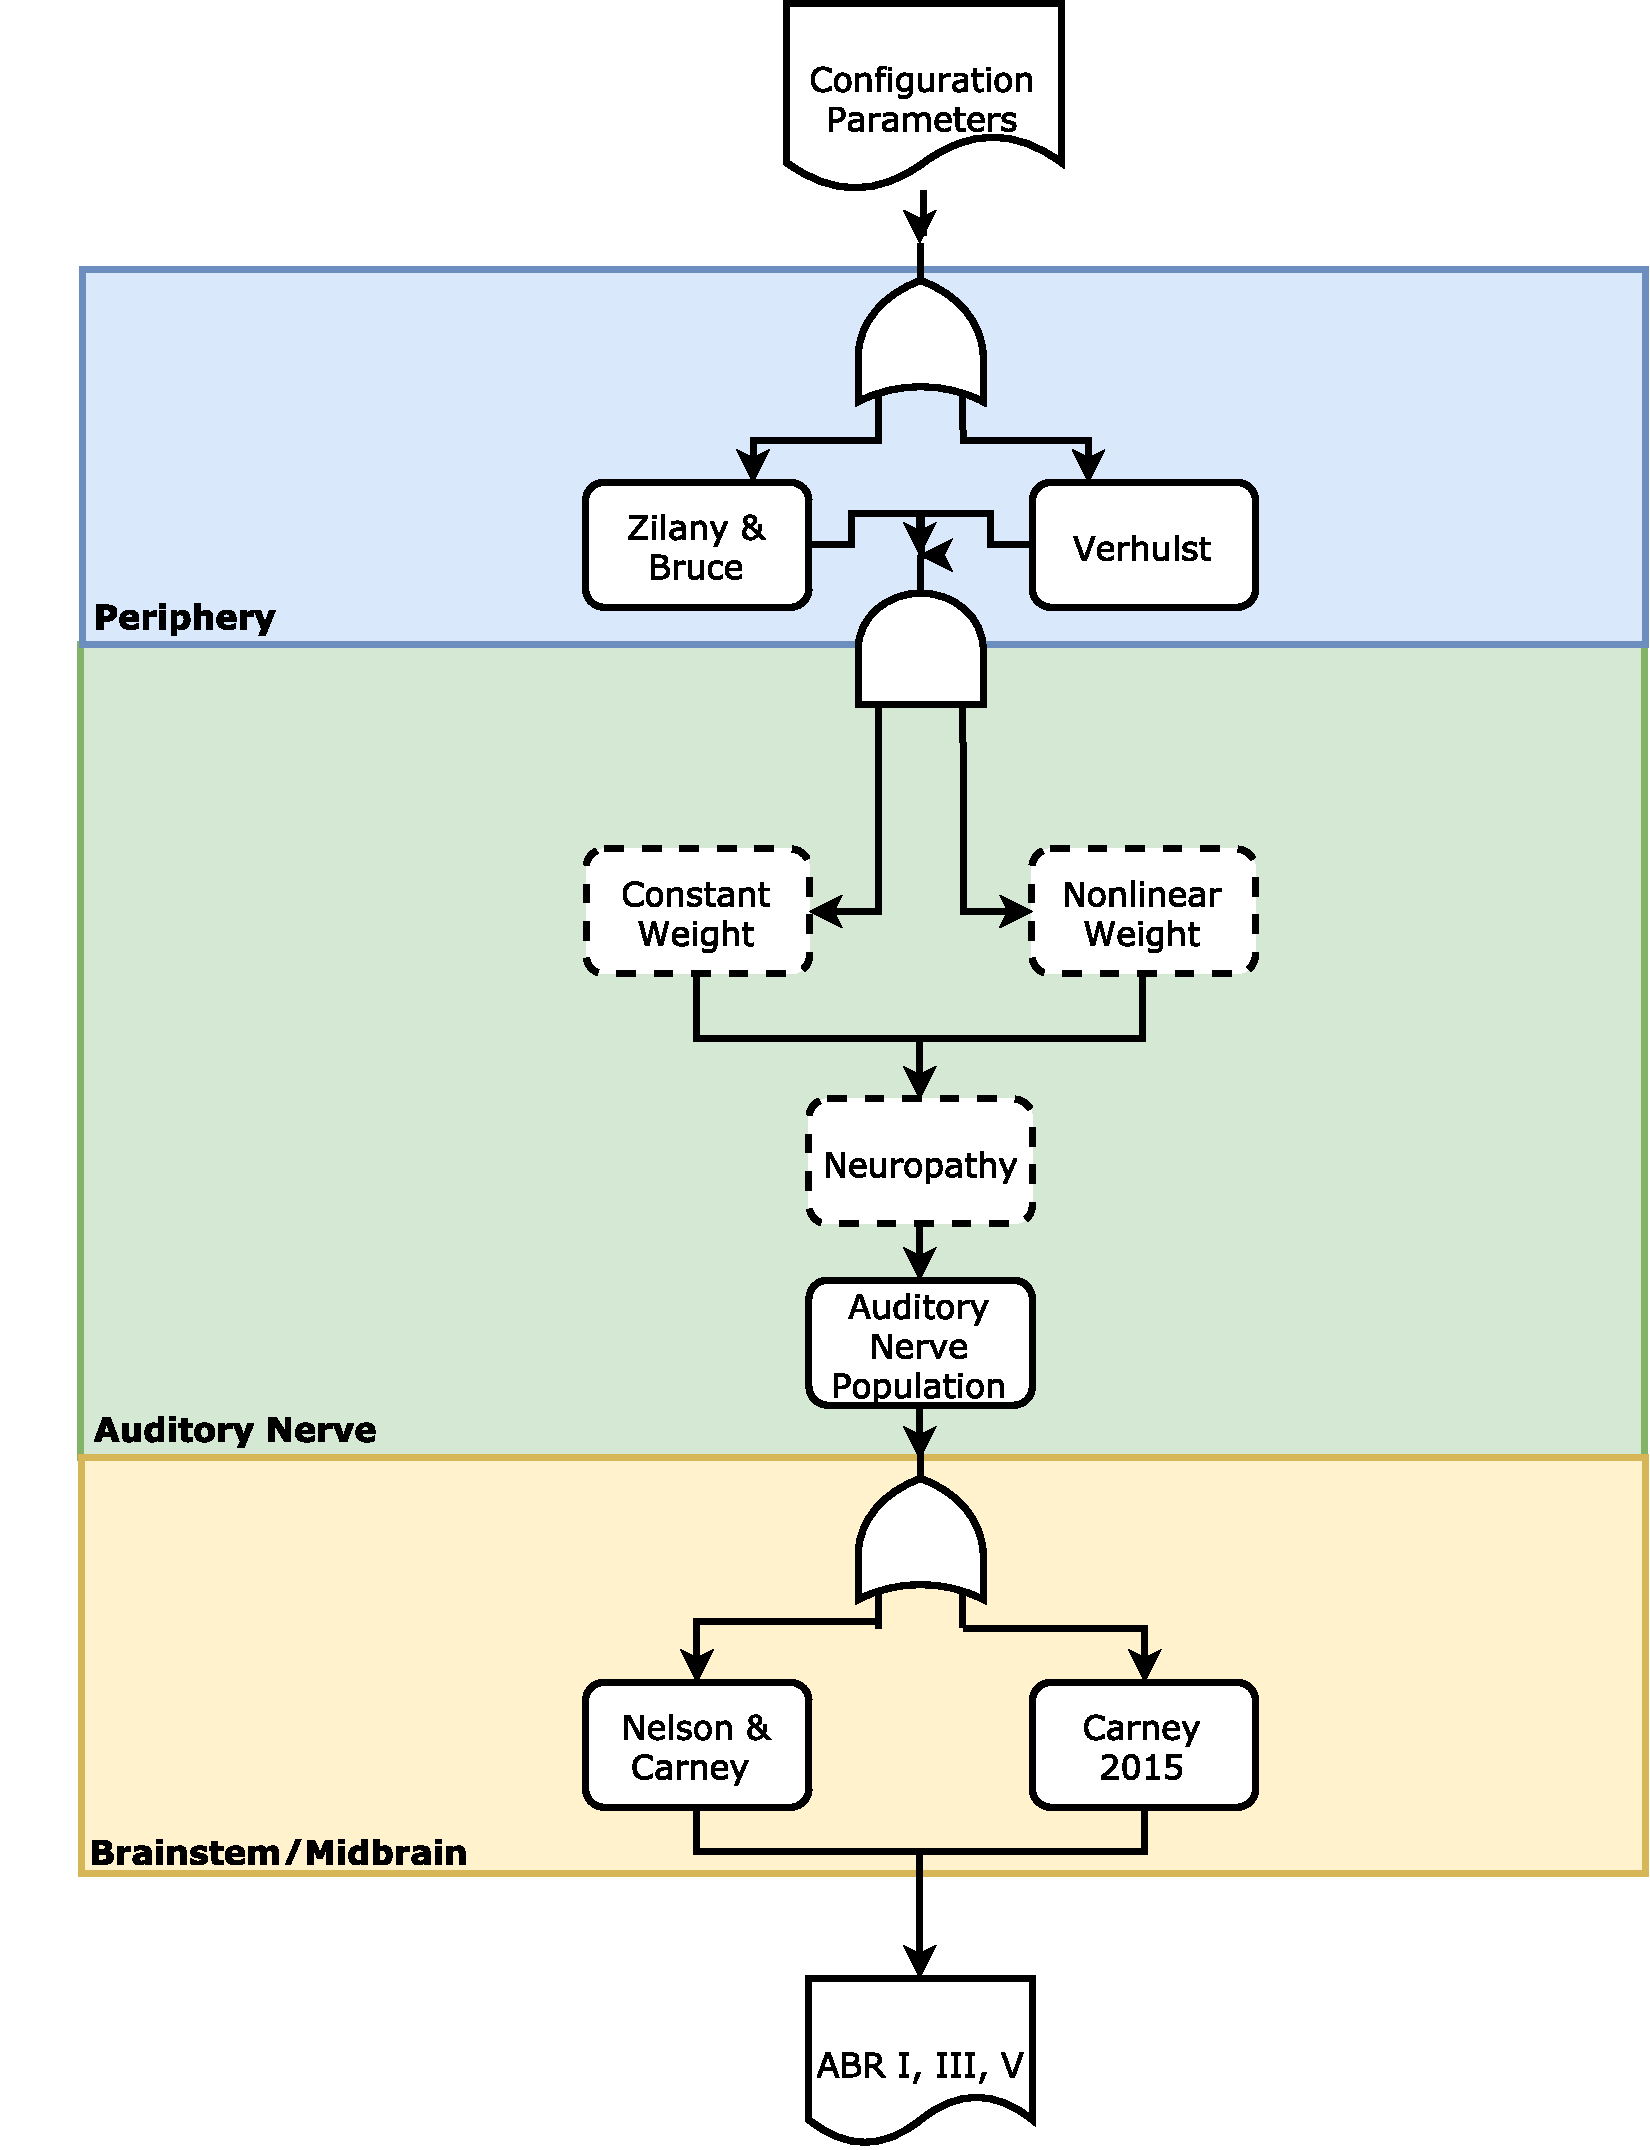
\includegraphics[width=0.95\textwidth]{high-level-overview.pdf}
	\caption[Overview of the Corti modeling environment.]{\textbf{Overview of the Corti modeling environment.} Two parameter trajectories are shown: a simulation of auditory neuropathy using the Verhulst periphery, nonlinear weights of fiber type contributions, and the Nelson and Carney brainstem (orange), and a simulation without neuropathy using the Zilany periphery, linear fiber weighting, and the Carney 2015 brainstem (red).}
	\label{fig:corti-overview}
	\end{figure}

\subsection{Model Parameters} % (fold)
\label{sub:model_parameters}

% subsection model_parameters (end)
% section overview_of_modeling_framework (end)
\section{Stimulus Generation} % (fold)
\label{sec:stimulus_generation}
Corti supports simulations of stimuli of arbitrary duration and level.  Simple stimuli such as clicks are generated programmatically by specifying a series of parameters such as onset time and duration, and more complex stimuli can be specified as WAV files.  All WAV stimuli must specify a sound level in dB SPL re 20$\mu$Pa; the waveform is then normalized by the peak value (in the case of a click) or the RMS value (for spectrally complex stimuli) and rescaled to have units of Pascals prior to simulation.
% section stimulus_generation (end)
\section{Peripheral Models} % (fold)
\label{sec:peripheral_models}
Two models of the auditory periphery are included: the transmission-line model by~\cite{Verhulst2015Functional} (henceforth ``The Verhulst model'') and the phenomenological model by~\cite{Zilany2014Updated} (henceforth ``The Zilany model'').

\subsection{The Verhulst Model} % (fold)
\label{sub:the_verhulst_model1}
The Verhulst model is useful for broadband stimuli.  It handles off-frequency effects (dispersion) well, and produces detailed information about many stages of sound propagation.  Otoacoustic emissions are also modeled. 

The theoretical background of the model is discussed in chapter 2.

Since the development of the Verhulst model is still underway, it has been programmatically isolated in a separate package.  This provides a separation of concerns between the projects, and allows both Corti and the Verhulst model to be updated independently of each other as new features are made available in both.
% subsection the_verhulst_model (end)
\subsection{The Zilany Model} % (fold)
\label{sub:the_zilany_model}
The implementation of the Zilany model here was adapted from~\cite{Rudnicki2014Cochlea}, who provided a Python and C implementation that has been shown to produce identical output to the version documented by~\cite{Zilany2014Updated}. 

% subsection interoperability_of_the_zilany_and_verhulst_models (end)
\subsection{Interoperability of the Zilany and Verhulst Models} % (fold)
\label{sub:interoperability_of_the_zilany_and_verhulst_models}
The classification of SR types differs between the Zilany and Verhulst models in their firing rate classification cutoffs.  For the purposes of this work, both support combining the low- and medium- rate fibers into one population with mean spike rates less than 18 spikes/sec.  


% subsection the_zilany_model (end)

\subsection{Peripheral Model Output} % (fold)
\label{sub:peripheral_model_output}
The Verhulst model provides estimates of response behavior at many stages of the of the auditory periphery.  The Zilany model provides some of the same.  

Both provide estimates of Instantaneous Firing Rate as a function of post-stimulus time for each combination of fiber type and best frequency, and these are passed to the next stage of the Corti environment.
% subsection peripheral_model_output (end)

% section peripheral_models (end)

\section{Auditory Nerve Response Models} % (fold)
\label{sec:auditory_nerve_response_models}
This stage of processing converts IFRs of specific fiber populations into an estimate of the summed activity of the auditory nerve. 

\subsection{Modeling Contributions of Inner Hair Cells} % (fold)
\label{sub:contributions_to_the_response_by_inner_hair_cells}
Along the Organ of Corti, each inner hair cell is innervated by multiple spiral ganglia.  The Verhulst and Zilany models, however, give responses of ``one'' fiber of each spontaneous rate type for each best center frequency, so modeling the summed response per IHC requires multiplicatively summing the responses of each SR type. 

Based on anatomical data (liberman 1978), the Verhulst model assigns 19 fibers to each inner hair cell.  

The Zilany model's output is summed accordingly. 
% subsection contributions_to_the_response_by_inner_hair_cells (end)
\subsection{Weighting of IHC contribution} % (fold)
\label{sub:weighting_of_ihc_contribution}
The Verhulst model applies a scalar weighting factor to the summed Auditory Nerve Response using an undamaged nerve with 19 total fibers per IHC with 3 fibers for Low and Medium SR fibers and 13 High SR fibers. The scalar weighting factor was empirally chosen such that the modeled and summed response of IHCs with CFs logarithmically spaced between 175Hz and 20kHz produces a model ABR Wave-1 amplitude of 15 $\mu$V.  \citeauthor{Verhulst2015Functional} found the value of this weighting factor to be \num{0.15e-6} V $\times$ \num{2.7676e-07}.

To produce comparable results, the Zilany model was scaled accordingly. By iteratively converging on a scaling factor with a tolerance of $\pm$1 nV, the scaling factor that produced an ABR Wave-1 amplitude of 15$\mu$V$\pm 1$nV was found to be \num{0.15e-6} V $\times$ \num{7.30282e-07}.
% subsection weighting_of_ihc_contribution (end)


\subsection{Weighting of Fiber Types per IHC} % (fold)
\label{sub:weighting_of_fiber_types_per_ihc}
Based on data from~\cite{Temchin2008Threshold}, the distribution of SR fiber types per IHC may not be uniform along the length of the basilar membrane.  To account for this, fiber types may be weighted per IHC, rather than kept at the fixed 3-3-13 ratio set by Verhulst.  
\begin{figure}[htbp]
	\centering
	%\includegraphics[width=0.95\textwidth]{}
	\caption{Curve-fitting of experimental results by Temchin}
	\label{fig:temchin-curvefit}
\end{figure}

The empirical fit equation that estimates the percentage of fibers innervating a given inner hair cell as a function of best frequency was found to be: 

\subsubsection{Fractional weights}
A consequence of the approach taken in section~\ref{sub:weighting_of_fiber_types_per_ihc} is that while the total fiber count per IHC is fixed at 19 fibers, the percentage of the summmed response of that IHC that arises from a given fiber type is no longer guaranteed to be an integer number of fibers.  Therefore, it is appropriate to think of such values as weighted contributions rather than individual spiral ganglia.  In the context of producing auditory nerve responses---as are used in this work---this can be thought of as providing a more accurate representation of \emph{summed} physiological responses. If the model response of individual unitary fibers is desired, the modeling environment saves individual fiber responses at the level of the periphery.
% subsection weighting_of_fiber_types_per_ihc (end)

\subsection{Modeling Synaptopathy} % (fold)
\label{sub:modeling_synaptopathy}
Selective degredation of the auditory nerve response is modeled by scaling each fiber type at each CF by a percentage factor.  

This will matter a lot when fiber types aren't linearlly allocated, and especially at high frequencies.
% subsection modeling_synaptopathy (end)
% section auditory_nerve_response_models (end)

\section{Brainstem Models} % (fold)
\label{sec:brainstem_models}
This section details the two brainstem models in use, given by~\cite{Nelson2004Phenomenological} and~\cite{Carney2015Speech}.

\subsection{The Nelson Carney 2004 Brainstem} % (fold)
\label{sub:the_nelson_carney_2004_brainstem}

% subsection the_nelson_carney_2004_brainstem (end)
\subsection{The Carney 2015 Brainstem} % (fold)
\label{sub:the_carney_2015_brainstem}

\subsubsection{Choice of Best Modulation Frequency}
Refer to laurel's EPL talk spring 2016 -- 100 Hz because it's physiologically relevant.  No ``MTF Bank'' because the science isn't there yet. Unclear how or why they'd affect wave V delays. 

% subsection the_carney_2015_brainstem (end)
% section brainstem_models (end)

\section{Automated Parameter Exploration} % (fold)
\label{sub:automated_parameter_exploration}
Corti may be run in one of two modes.  In the first, a single set of parameters defines a single trajectory and the model is run once.   However, while this mode of operation is convenient for fast simulations whose parameters can be defined \emph{a priori}, it rapidly becomes impractical for situations where the relative effects of different parameter choices are to be compared, and reliable book-keeping of which parameters were used to generate which results becomes unnecessarily challenging.

Therefore, a second means of use was created, as detailed in \autoref{fig:pypet-overview}.  It provides a convenient interface to explore the parameter space generated by the specification of many available models, impairments, and options in a manner that allows easy \emph{post-hoc} analysis. Individual trajectories may be computed in parallel on a single workstation or in a high-performance cluster so that the relative effects of each model, neuropathic impairment, and other features may be directly compared.  The results for all combinations of model components are stored in one Hierarchical Data Format (HDF5) file.  Comparisons of the effect of using different trajectories to the same stimuli can then be made in a way that guarantees an internally consistent analysis.

The core of this mode is the Python library 

\begin{figure}[htbp]
	\centering
	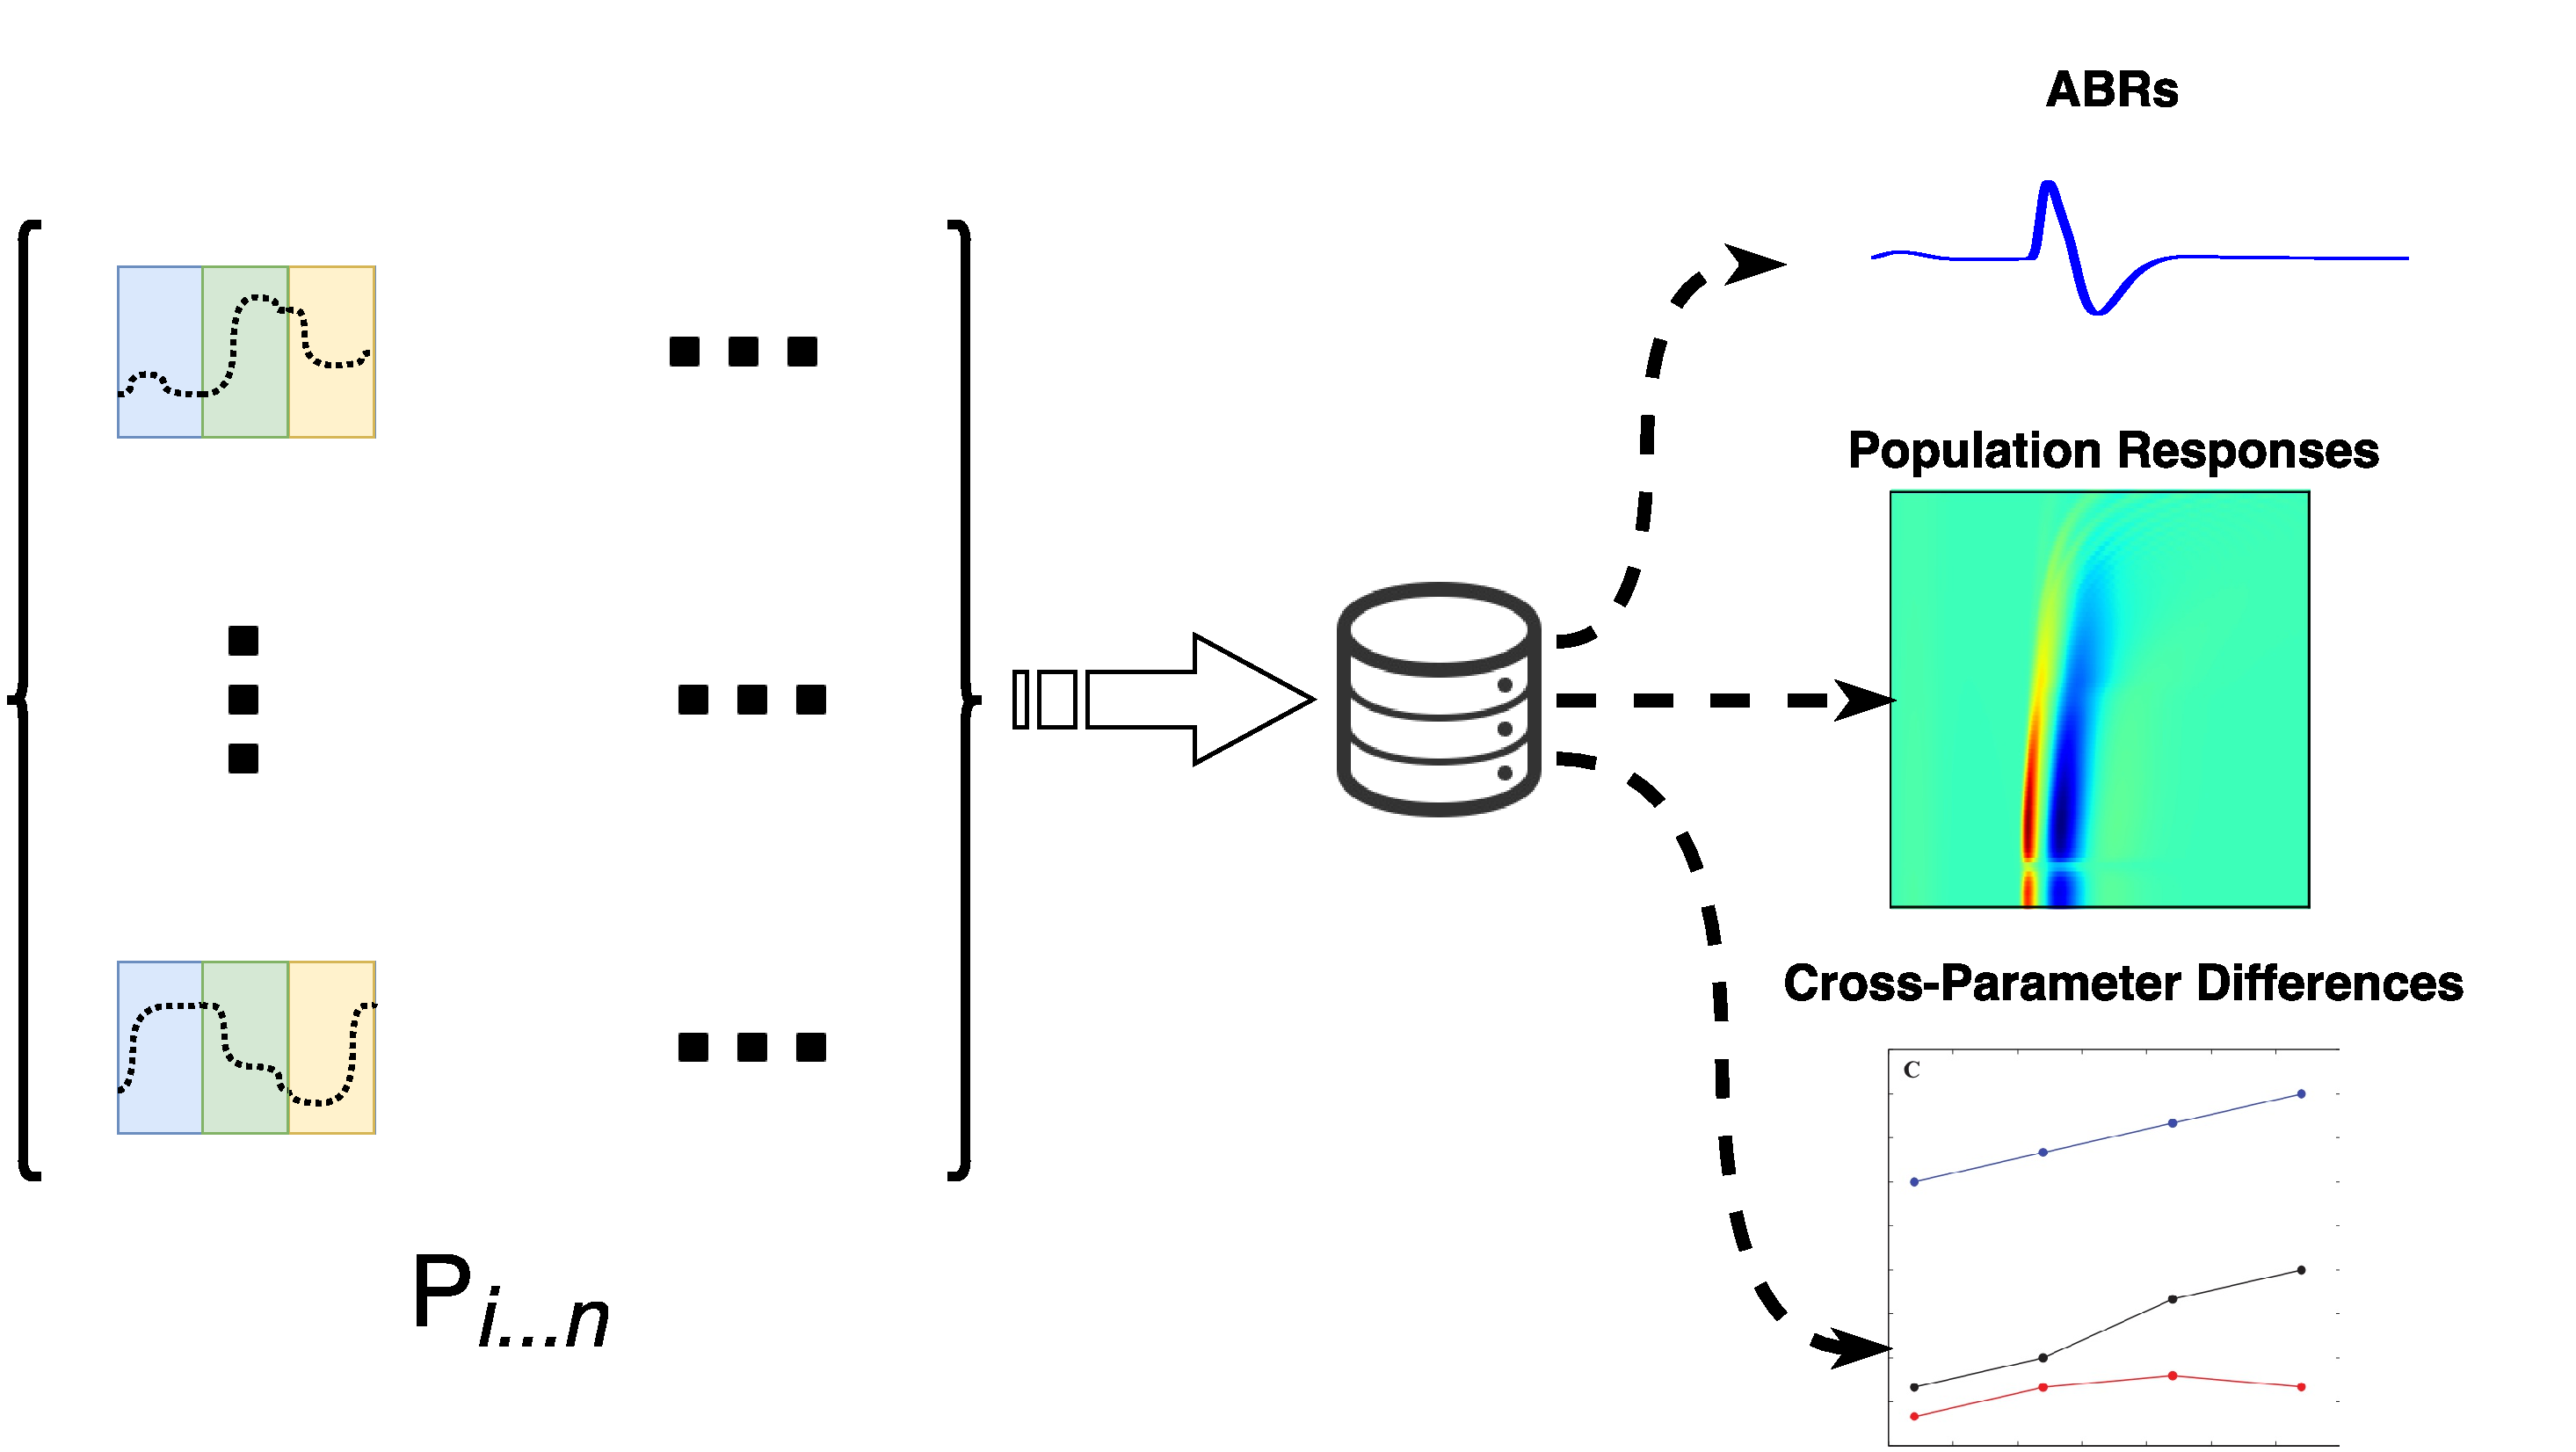
\includegraphics[width=0.95\textwidth]{pypet-workflow.pdf}
	\caption[Automated exploration of model parameters]{\textbf{Automated exploration of model parameters} P$_i$ is the set of parameters required to specify one trajectory.  $N$ trajectories, where $N$ is the cartesian product of the specified value ranges that a given parameter may take, are computed in parallel and stored in a database for further analysis. }
	\label{fig:pypet-overview}
\end{figure}
\subsection{Design of new experiments} % (fold)
\label{sub:design_of_new_experiments}

% subsection design_of_new_experiments (end)
% subsection automated_parameter_exploration (end)
% section usage_of_the_modeling_environment (end)